%----------------------------------------------------------------------------------------
%	PACKAGES AND OTHER DOCUMENT CONFIGURATIONS
%----------------------------------------------------------------------------------------

\documentclass[paper=a4, fontsize=11pt]{scrartcl} % A4 paper and 11pt font size
\usepackage{multicol}
\usepackage[T1]{fontenc} % Use 8-bit encoding that has 256 glyphs
\usepackage{fourier} % Use the Adobe Utopia font for the document - comment this line to return to the LaTeX default
\usepackage[english]{babel} % English language/hyphenation
\usepackage{amsmath,amsfonts,amsthm} % Math packages
\usepackage{listings}
\usepackage{lipsum} % Used for inserting dummy 'Lorem ipsum' text into the template
\usepackage{graphicx}
\usepackage{subfig}
\usepackage{float}

\usepackage{sectsty} % Allows customizing section commands
\allsectionsfont{\centering \normalfont\scshape} % Make all sections centered, the default font and small caps

\usepackage{fancyhdr} % Custom headers and footers
\pagestyle{fancyplain} % Makes all pages in the document conform to the custom headers and footers
\fancyhead{} % No page header - if you want one, create it in the same way as the footers below
\fancyfoot[L]{} % Empty left footer
\fancyfoot[C]{} % Empty center footer
\fancyfoot[R]{\thepage} % Page numbering for right footer
\renewcommand{\headrulewidth}{0pt} % Remove header underlines
\renewcommand{\footrulewidth}{0pt} % Remove footer underlines
\setlength{\headheight}{13.6pt} % Customize the height of the header

%\numberwithin{equation}{section} % Number equations within sections (i.e. 1.1, 1.2, 2.1, 2.2 instead of 1, 2, 3, 4)
%\numberwithin{figure}{section} % Number figures within sections (i.e. 1.1, 1.2, 2.1, 2.2 instead of 1, 2, 3, 4)
%\numberwithin{table}{section} % Number tables within sections (i.e. 1.1, 1.2, 2.1, 2.2 instead of 1, 2, 3, 4)

%\setlength\parindent{0pt} % Removes all indentation from paragraphs - comment this line for an assignment with lots of text

%----------------------------------------------------------------------------------------
%	TITLE SECTION
%----------------------------------------------------------------------------------------

\newcommand{\horrule}[1]{\rule{\linewidth}{#1}} % Create horizontal rule command with 1 argument of height

\title{	
\normalfont \normalsize 
\textsc{Syddansk Universitet} \\ [25pt] 
\horrule{0.5pt} \\[0.4cm] % Thin top horizontal rule
\huge SVM and Neural Networks \\ % The assignment title
\horrule{2pt} \\[0.5cm] % Thick bottom horizontal rule
}

\author{Bjarki Sigurdsson \\ Abdulrahman Abdulrahim \\ Miguel de la Colina \\ Group 5}
 % Your name

\date{\normalsize\today} % Today's date or a custom date

\begin{document}

\maketitle % Print the title

%----------------------------------------------------------------------------------------
%	PROBLEM 1
%----------------------------------------------------------------------------------------


\section*{Abstract}

\paragraph{The purpose of the exercise was to get familiar with neural network and support vector machines and to get a grasp of how they work and how they function when using real data-sets in this case the ciphers.}
%The purpose of this report is to use the k-nearest neighbor algorithm on a data-set made of ciphers. We will be dividing the data into two sets, one for training and one for testing. We will analyze the results for different values of k and DPI to see how this alters our results. Also we will be applying the  Gaussian smoothing with various sigmas in order to see how does this alter the results.}  

%------------------------------------------------


%----------------------------------------------------------------------------------------
%	PROBLEM 2
%----------------------------------------------------------------------------------------

\section{Neural Networks}
	For this exercise we use two-person data, reduced to the first 5 PCs and then split 50-50 to person-dependent training and test sets. We experiment with varying hidden layer structure as well as learning rates. We use the RSNNS package with \texttt{Std_Backpropagation} learning and a maximum of 1000 iterations throughout. For classification, we choose the output with the highest value in a winner-takes-all manner.\par
	We train a neural network using the package's \texttt{mlp} function and plot it using a custom function from \footnote{\url{https://gist.githubusercontent.com/fawda123/7471137/raw/466c1474d0a505ff044412703516c34f1a4684a5/nnet_plot_update.r}}. The resulting network is shown in figure \ref{fig:nn}. We also plot its error for each iteration as shown in figure \ref{fig:iterr}. We see that this error converges with time as the network reaches a local minimum error.

	\begin{figure}[h]
		\centering
		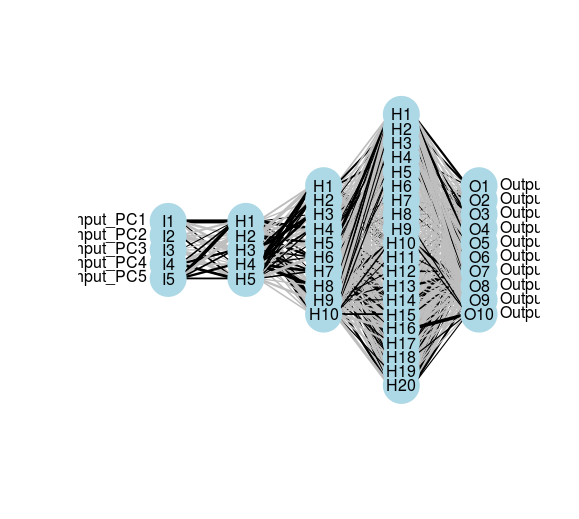
\includegraphics[width=0.8\textwidth]{nn.png}
		\caption{Neural network with hidden layer sizes c(5, 10, 20).}
		\label{fig:nn}
	\end{figure}

	\begin{figure}[h]
		\centering
		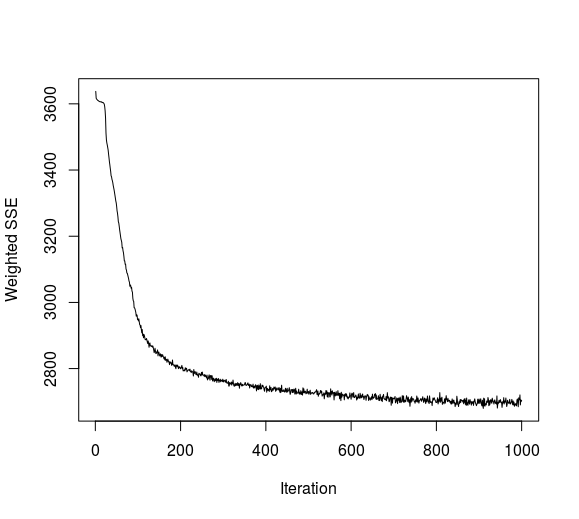
\includegraphics[width=0.8\textwidth]{iterr.png}
		\caption{Neural network with hidden layer sizes c(5, 10, 20).}
		\label{fig:iterr}
	\end{figure}

	\newpage
	The results for varying the hidden layer sizes and learning rates are shown in table \ref{tab:vary}. \par
	We see that there is a lot of freedom in the structure as various different structures yield similar results. We also see that there is a minimum number of neurons required for reasonable results. We also see that depth alone does not yield better results.\par
	Learning rate affects the rate of gradient descent during training. A high learning rate will lead to fast convergence but may overlook local minima. A lower learning rate, by comparison, will require more iterations to converge. In our case, both learning rates result in the network converging to similar error rates.

	\begin{table}[h]
	\centering
	\caption{Varying structure and learning rate.}
	\label{tab:vary}
	\begin{tabular}{l|l|l}
	Hidden Structure                 & Learning Rate & Accuracy \\ \hline
	c(1)														 & .2						 & .15325		\\
	c(5,10,20)                       & .2            & .4255    \\
	c(10, 20)                        & .2            & .49525   \\
	c(20, 40)                        & .2            & .48975   \\
	c(10,10,10,10,10,10,10,10,10,10) & .2            & .098     \\
	c(100)                           & .2            & .4985    \\
	c(200)                           & .2            & .4905    \\
	c(100)                           & .1            & .49525   \\
	c(100)                           & .7            & .4935   
	\end{tabular}
	\end{table}


\clearpage
\section{SVM}


\end{document}
\grid
